\chapter{Introduction} \label{chap:intro}

\section*{}

This chapter presents the context and motivation of this thesis, describing the main goals, its objectives and the expected results.

\section{Context and motivation} \label{sec:context}

Nowadays current markets are changing, we can see more often the globalization phenomenon and with that organizations are compelled to streamline their business in order to achieve a favorable market position and be able to maintain or increase their competitiveness.

In our everyday lives software takes an important role, it is everywhere and is needed more often. When is in development is important to make it more efficient and with more quality. For software development organizations failures and errors are not allowed and each one of them implies increased costs and resources being wasted. To avoid this scenario and to achieve maximum efficiency and agility, their processes and their methodologies need to be less time consuming and more effortless so good practices need to be followed in order to allow them focus on what really matters: value creation. This will provide them advantages and make them more trustful.

Organizations need to ensure that their products and services consistently meet customer’s requirements, and that quality is consistently improved and certifications are a formal recognition of those ideals. Sadly those recognitions take too much time and effort and in some cases they are very painful and expensive.

Capability Maturity Model Integration(CMMI)\citep{CMMI} is a framework of best practices and does not describe the processes themselves, it describes the characteristics of good processes in order to improve organizations and is required by many U.S. Government contracts, especially in software development.

SCAMPI is the Standard CMMI Appraisal Method for Process Improvement and it provide benchmark quality ratings relative to CMMI models.

SCRAIM is a life cycle and project management tool developed by Stronstep combined with process management techniques. It is going to provide the background and the base to work and simplify those kind of evaluations in order to save time and money. That way companies will deliver their products and services better, faster, and cheaper.

\section{Goals and expected results} \label{sec:goals}

The main goal is of this dissertation is to develop a group of methodologies, techniques and tools integrated in the SCRAIM, that will make evaluations and certain parts of certifications easier and less painful for the SCRAIM users.
Although there are a number of life cycle and project management tools, few combine this with process management techniques. SCRAIM combines the two and will provide the users new features that will semi-automate the assessment for certification of an organization. 


%\begin{figure}[h]
%	\begin{center}
%		\leavevmode
%		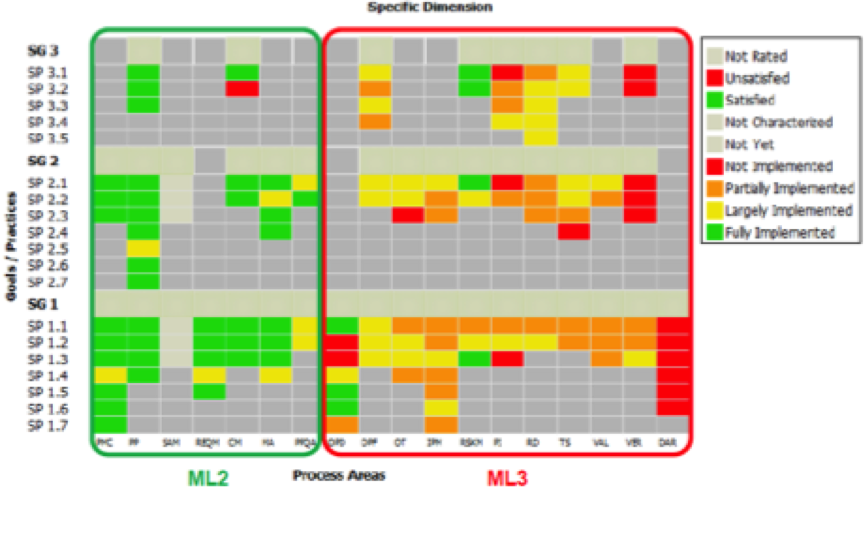
\includegraphics[width=0.86\textwidth]{thesis_goals}
%		\caption{SCAMPI results}
%		\label{fig:arch}
%	\end{center}
%\end{figure}

More specifically, the goals of this dissertation work are as follows: 

\begin{enumerate}[i]%for capital roman numbers.
	\item Analyze to what extent the SCRAIM tool supports the implementation (including the collection of evidences) of the specific practices of CMMI-DEV for maturiy levels 2 and 3 (ML2-3), and recommend relevant improvements to SCRAIM;
	\item Define rules to automatically assess the degree of fulfillment of CMMI-DEV ML2 practices by SCRAIM users, by analysing organizational project data and any other relevant evidences recorded in SCRAIM;
	\item For the practices  of CMMI-DEV ML2 that cannot be assessed automatically, define questionnaires to assist the users in doing a manual assessment;
	\item Implement in SCRAIM rules and questionnaires defined in steps (ii) and (iii), for some process areas, including appropriate user interfaces to conduct assessments and visualize assessment results;
	\item Validate the electronic assessment approach in real world projects.
\end{enumerate}

The full-automated process is not yet feasible, so human intervention is still mandatory. With the use of SCRAIM, good practices will be followed and in the end the generated information will facilitate the decision making process. We can see many advantages of this innovation, and we believe that the application of this innovation will help reducing the costs and time of one evaluation using the SCAMPI method.

\section{Document structure} \label{sec:Structure}

This document is divided into six main chapters. The first and present chapter serves as an introduction where is presented the context and motivation for this thesis and also the goals and expected results to be delivered.

In chapter 2 is made a problem analysis, giving insight about CMMI, SCAMPI and the tool to be used SCRAIM.

Chapter 3 presents the state of the art and related work regarding electronic assessment. It are described in detail the most used and most important tools that are currently being used in the appraisals.

In chapter 4 is clarified the scope of the project and in chapter 5 is made a description of the found solution.

The chapter 6 presents an example of usage and experimentation of the developed solution.

The final chapter is makes a resume of the document, presents the final conclusion and future work.